
\maketitle

\begin{abstract}
In the life-cycle of objects there are different phases. The phase in which an object currently is, affects how it is handled in an application; however these phase shifts are typically implicit.
In this study we propose a new language mechanism, called instance pointcuts, based on aspect-orientation.
They maintain sets of objects according to events in their life-cycle and create notifications when new objects are added or removed from the set.
The selection criteria of instance pointcuts can be refined, e.g., to define a subset or super-set of an existing instance pointcut; and they can be composed, e.g., by set operations.
Our approach improves modularity by providing a fine-grained mechanism and a declarative syntax to maintain a set of objects.
\end{abstract}

\section{Introduction}
In object-oriented programming (OOP), objects encapsulate state and behavior; objects also have a life-cycle, which means that the same object can play different roles at different times. And which role an object is currently playing is important as it can affect the object's own behavior or how objects are handled. Typically the shift from one life-cycle phase to another is implicit, e.g., determined by passing an object from one client to another. In this paper, we propose a new language mechanism for declaratively specifying life-cycle phases and for exposing the set of objects which are currently in a specific phase. This declarativity allows us to give guarantees about these sets like subset relationships, as well as to perform compile-time checks like warning about sets that will always be empty.

As an example of different relevant phases in the life-cycle of objects, consider an online store application. Assume that the offered products are objects in the program and that specific budget plans should be offered for products depending on their life-cycle phase. A first example of such a phase is a period during which a product is in the wish-list of any customer; this phase begins when ``product'' object is added to the ``wish-list'' property of a ``customer'' object and it ends when it is removed from this property. A second example is the phase when an object is out of stock. Thus, we defined two sets of objects: the set of objects into which at least one customer is interested and the set of objects that are sold out. Finally, the shop owner may be interested in the intersection of these sets and give priority to reordering the corresponding products.

Furthermore, in OOP objects are categorized according to their \emph{types}.
This is a structural categorization and it does not give any information about the events that object participates in.
However, grouping objects according to another criteria such as, the class they were initialized in or being passed as an argument to a certain method would only be possible by inserting code at those particular points, which would litter the code.

To be able to process the objects which are currently in a relevant life-cycle phase (like having been added to a wish-list), bookkeeping is required to keep track of the set. To separate this bookkeeping code from the business logic of the program, aspect-oriented programming (AOP) is a well known technique. But in AOP, \emph{pointcuts} select sets of so-called \emph{join points} which are points in time during the execution of the program; current aspect-oriented languages do not offer dedicated mechanisms for selecting \emph{sets of objects}.

These languages do not support a \emph{declarative specification} of the objects belonging to a life-cycle phases; instead an \emph{imperative implementation}, always following the same pattern, is required for collecting those objects.
A consequence of such an imperative solution, besides all the negative effects of hand-writing boilerplate code, is that automatic reasoning becomes practically impossible.
In addition, a declarative implementation makes the relevant information explicit, which reduces checking efforts as well as making the code readable.

To offer better support for processing objects according to their life-cycle phase, we propose a language construct that builds on the technology of aspect-orientation.
We borrow the terminology and provide \emph{instance pointcuts} to select sets of objects based on the execution history.

An instance pointcut definition consists of three parts: an identifier, a type which is the upper bound for all objects in the selected set, and a specification of relevant objects.
%Instance pointcuts do not have any parameters, the only information that is explicitly given is the \emph{type} of the instance we are interested in selecting.
The specification consists of two \emph{pointcut expressions} that select relevant join points in the objects' life-cycle and expose the object: the mark the beginning and end of a life-cycle phase; i.e., the object is added to or removed from the set.

New instance pointcuts can be derived from existing ones. One instance pointcut can be declared to be a \emph{subset} or a \emph{super-set} of an existing one.
In this case, the specification of the life-cycle phase is narrowed down or broadened, respectively.
%One way is to refer to an instance pointcut and \emph{co-variantly} refine its selected type. Another way is to This composition mechanism is strengthened with the ability to declaratively define a pointcut as a \emph{subset} or a \emph{super-set} of another one. These relationships come with additional checks which ensure that there are no inconsistencies between a super-set and its subsets, such as a subset containing instances that are not members of its super-set.
Composition of existing instance pointcut is also supported in terms of set operations: \emph{intersection}, \emph{union} and \emph{set difference}. 

%, and the exposed variable is added to the set. It is also possible to remove object from the set and this is done via the \emph{de-selection} expression which is also defined in the form of a pointcut expression. When the expression is evaluated to be true, if the exposed instance exists in the set then it is removed. It is possible to point to certain places at join-points via using before and after clauses. With this feature it is possible to select instances before they are passed as an argument or after they call a method. 


\section{Motivation - Example Section}
\label{sect:motivation}

Objects can be categorized by how they are used (passed as arguments to method calls, act as receiver or sender for method calls, etc.). Concerns may be applicable to objects used in the same way. Therefore we must be able to identify and select those objects that are similarly used. Since object behavior is the building block of system behavior, such a categorization will allow behavior extensions on the object-level, providing an extra dimension of modularity.

\begin{figure}[h]
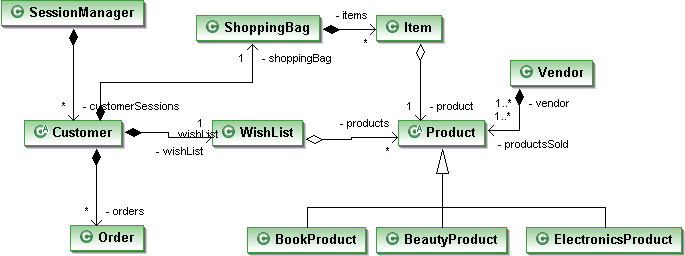
\includegraphics[width=\textwidth]{images/myonlineshop.png}%
\caption{A simple online shop application}%
\label{fig:shop}%
\end{figure}

In the remainder of this section we outline the architecture and design of an online store application. Then we use this scenario to give examples of categorizing objects according to how they are used and how to use these categories in the implementation of unanticipated concerns. Finally we conclude requirements for solving the encountered challenges in these examples.

\paragraph{Online Shop}
An online shop is a sophisticated web application and objects of the same type can exist at different stages of the control flow. In Figure \ref{fig:shop} the static structure of a simplified online shop is shown. When a new user logs in, \texttt{SessionManager} creates a \texttt{Customer} object to represent the user's session. A customer has a \texttt{ShoppingBag} and a \texttt{WishList}. The abstract class \texttt{Product} is super-type of all products in the shop and represents product data. The \texttt{Product}'s subclasses are \texttt{BeautyProduct}, \texttt{BookProduct} etc. When the customer selects a product and clicks add to shopping bag, an new \texttt{Item} instance is created and added to the \texttt{ShoppingBag} object; the \texttt{Item} instance contains the \texttt{Product} and how many of that \texttt{Product} was added. A customer can add/remove items from his shopping bag. When the shopping is finished then the \texttt{checkOut()} method is invoked, which returns an object of type \texttt{Order}. To complete the order the customer has to provide some information and finalize the order. A \texttt{Customer} can olso wishlist \texttt{Product}s by adding them to his \texttt{WishList}; the \texttt{WishList} holds a list of \texttt{Products} (whereas \texttt{ShoopingBag} holds a list of \texttt{Item}s).


Let's assume a new requirement for applying a happy-hour discount is introduced. The discount should apply to a set of \texttt{Item}s which are selected when they exist in the context of an interesting event. The new requirement is as follows, \textsf{when a customer adds items to his shopping bag between certain hours, then those items will be applied a discount in check out}. In order to realize this in an OO-approach, one needs to insert the code regarding the discount concern, to the place where the event of interest occurs.
%For the following discount rule; \textsf{when an item is added to a shopping bag between certain hours, then they are applied the happy-hour discount}, 
With an OO-approach, to satisfy the new requirement we need to invasively change the system code. First we need to keep a list of items that were added to shopping bag inside the timing condition. Then when the user finally checks out, we should apply the discount to the items in the list. Listing \ref{lst:happyhour} shows that we need to insert code in multiple places to satisfy the new requirement. First a set, called \texttt{happyItems}, is created (Line 1), to keep track of items that are added during the happy-hour. In \texttt{addToShoppingBag} method a if statement checking the timing condition is defined, when the condition is true than the created item is added to \texttt{happyItems} (Line 6-7).  Finally in the \texttt{checkOut} method the discounts are applied to the items in \texttt{happyItems} (Line 18-19). 

\begin{lstlisting}[float, caption={A Java implementation of Happy-hour discount rule}, label={lst:happyhour}]
Set<Item> happyItems = createSet();
public boolean addToShoppingBag(Product p, int amount)
{
	Item item = ItemFactory.createItem(p,amount);
	
	if('timing condition')
		items.put(item)
	
	this.shoppingBag.add(item);
}
public boolean removeFromShoppingBag(Item item, int amount)
{
	...
	items.remove(item);
}
public checkOut()
{
	foreach(i in happyItems)
		ProductManager.applyDiscount(i, DiscountRule.get(HAPPY_HOUR));
}
\end{lstlisting}

Even for a single discount rule, the code for the discount concern and the book-keeping that comes with it creates cluttering. If we would like to apply multiple discount rules for the \emph{check out} event, this way of implementing is clearly not suitable. Also this event may not be the only event we want detect for applying discount rules and the OO implementation will eventually be scattered and tangled. An aspect-oriented implementation can offer a better solution, by encapsulating the concern in an aspect. In Listing \ref{lst:happyhouraop} the \texttt{newItem} pointcut (Line 2-4) selects join-points where after customer adds a product to his bag, a new \texttt{Item} is created in \texttt{addtoShoppingBag} method. The advice is executed when \texttt{newItem} is matched; after returning the new item, the timing condition is checked and if it hols than the item is added to \texttt{happyItems}. We also define a \texttt{removeItem} pointcut (Line 5-7)  to remove an item from \texttt{happyItems} if it is removed from shopping bag. Finally, we define a pointcut for selecting the \texttt{Customer.checkOut()} join-point (Line 8) and before the method is executed we apply the discount to items in \texttt{happyItems}. AO implementation, although offers a non-invasive solution, also suffers from boilerplate code written for book-keeping. 

\begin{lstlisting}[float, caption={An Aspectj implementation of Happy-hour discount rule}, label={lst:happyhouraop}]
Set<Item> happyItems = createSet();
pointcut newItem(Item item): 
		call(* ItemFactory.createItem(..)) && 
		withincode(* Customer.addToShoppingBag(..));
pointcut removeItem(Item item): 
	call(* Customer.removeFromShoppingBag(..)) && 
	args(item);
pointcut checkOut(): call(* Customer.checkOut());

after() returning(Item item): newItem(item)
{
	if('timing condition')
		happyItems.put(item);
}
after(Item item): removeItem(item)
{
	happyItems.remove(item);
}
before():checkOut()
{
	foreach(i in happyItems)
		ProductManager.applyDiscount(i, DiscountRule.get(HAPPY_HOUR));
}
\end{lstlisting}

Let's look at another new requirement, which is as follows: \textsf{Keep a set of products that are currently out of stock,  once they become available raise an event and remove them from the set}. This scenario also requires when a condition holds and the set is changed there should be an event raised which means the set should be monitored. This creates an additional concern. 

Reusing existing sets by finding their subsets or composing them with set operations is also impractical with imperative programming. If we want to find the subset of \texttt{BeautyProduct}s in a set of \texttt{Product} objects, we have to iterate over it and check instance types to create a new set. Implementing set operations such as intersection also results in further boilerplate code.

In order to overcome the shortcomings of existing approaches, we need a way to declaratively select objects based their life-cycle phases, where the beginning and the end of a phase is marked by events. From the scenarios described above, we conclude the following requirements:

\begin{enumerate}[{Requirement}1{:}]
\item Provide a declarative way of reifying a set of objects by defining add/remove conditions
\item Support multi-sets, an object can be added multiple times
\item Add/Remove expressions select events and the object is exposed from the context of this event
\item Access the set of objects which is currently selected and be notified when the set changes
\item Provide a declarative way to refine existing sets to their subsets
\item Compose sets via set operations (intersection, union, set difference)
\item Provide checks for validity of composition, empty sets and subset-superset compatibility
\end{enumerate}
